\documentclass[10pt]{article}

%%%%%%%%%%%%%%%%%%%%%
% Package Inclusion %
%%%%%%%%%%%%%%%%%%%%%
\usepackage{geometry,amsmath,amsthm,mathrsfs,amssymb,graphicx,bm,hyperref,url}

%%%%%%%%%%%%%%%%%%%
% Custom Commands %
%%%%%%%%%%%%%%%%%%%
\newcommand{\n}{\noindent}
\newcommand{\norm}[1]{\left|#1\right|}
\newcommand{\avg}[1]{\left<#1\right>}

%%%%%%%%%%%%%%%%%%%%%%%%%%
% Title Page Information %
%%%%%%%%%%%%%%%%%%%%%%%%%%

\title{Notes for PHYS 232: Stellar Structure}
\author{Bill Wolf}
\date{\today}

\begin{document}

\vfill\maketitle\vfill \newpage

\tableofcontents \newpage

%%%%%%%%%%%%%%%%%%%%%%
% January 9, 2012 %
%%%%%%%%%%%%%%%%%%%%%%

\section{Introduction}
	\emph{Monday, January 9, 2012}
	\subsection{The HR Diagram} 
	Most stars shine predominantly in the optical range of the electromagnetic spectrum. As a result, we get most of our information about stars by observing their optical output.  It makes sense, then, that we might organize stars by there color, which is indicative of their surface temperature. When plotting a population of stars' luminosities against their surface temperature, we note a strong correlation between the two. As it turns out, the controlling parameter for these quantities is the mass of the star, at least while the star is on the \textbf{Main Sequence} (stars burning hydrogen to helium). The correlation between the mass of a main-sequence star and its luminosity is incredibly strong (see HR diagram examples).
	\begin{figure}
		\centering
		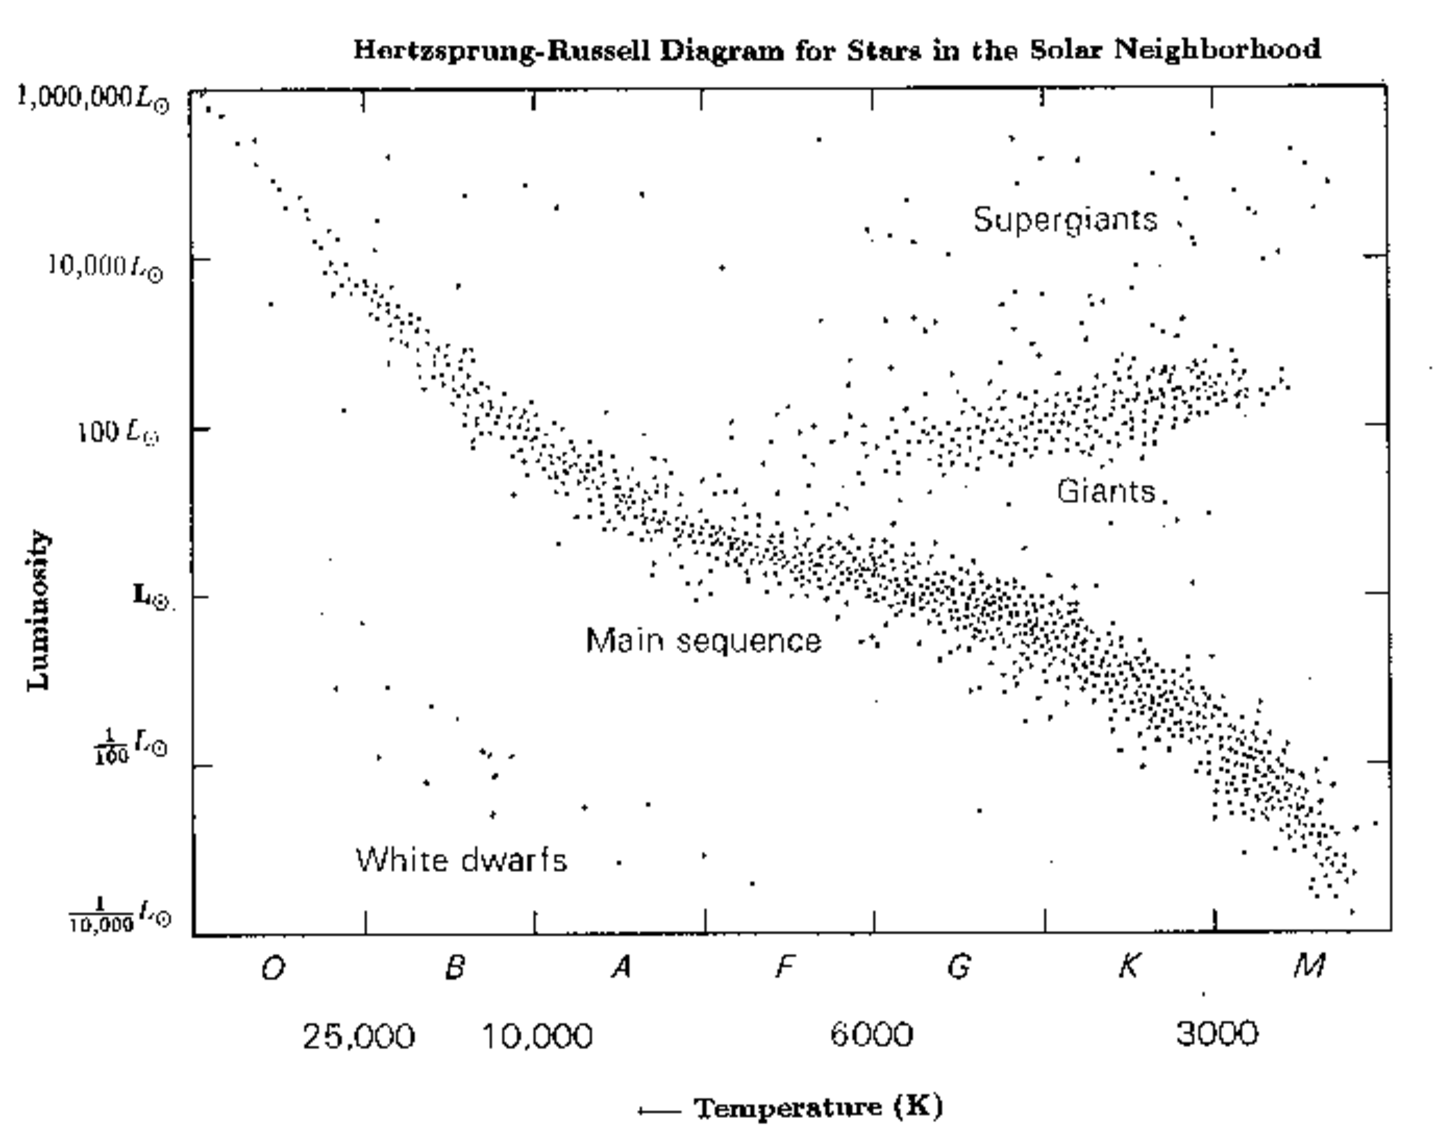
\includegraphics[width=6in]{hr_local.pdf}
		\caption{An HR diagram for stars in the local neighborhood (shamelessly stolen from Google Images)}
		\label{HR.1f}
	\end{figure}
	\subsection{Conditions for a Star on the HR Diagram}
	We are interested in knowing what defines the regime where a star can reside in a particular $L,\,T_{\mathrm{eff}}=[L/(4\pi\sigma_{\mathrm{SB}}R^2)]^{1/4}$. Why, for example, is there a dynamical range in the luminosity spanning over six orders of magnitude, while only a range of a factor of about 5 in the effective temperature? To gain some perspective, we might observe the number of stars as a function of brightness. We organize these stars by their \textbf{spectral type} (a rough measure of how big the star is) and find their approximate \textbf{mass density} (the amount of mass contained in these stars per unit volume):
	\begin{center} 
	\begin{tabular}{l l}
		Spectral Type & $\rho\ (M_\odot/\mathrm{pc^3})$\\
		\hline
		O-B & 0.4\\
		A-F & 4\\
		G-M & 40\\
		WD's & 20
	\end{tabular}
	\end{center}
	Here we've used the standard labels for different spectral types, O, B, A, F, G, K, M, L, T, which are roughly in decreasing order of size and temperature (the reasoning for this scale is historical rather than logical, and the ordering is often remembered by the mnemonic, ``Oh Be A Fine Gal/Guy, Kiss Me! Less Talk!''). We see that the big, bright stars form an exceedingly small portion of the amount of stellar mass in our galaxy. We will find that this is because large stars exhaust their fuel much more quickly than smaller stars, and thus live and die much faster. We'll now observe another type of classification of stars used in our neighborhood, the Milky Way Galaxy.
		
	\subsubsection{Population I Stars}
	From Earth, the center of the galaxy is approximately 8.5 kpc away. Meanwhile, the disk is only about 100 pc wide.  We've observed that stars in the thin disk (commonly known as \textbf{Population I Stars}) are orbiting at the orbital velocity with only a small amount of axial and radial motion. They are essentially dynamically cold and in nearly circular orbits. This is indeed where most of the \textbf{interstellar medium} (ISM) resides, causing much of the star formation in the galaxy. This region is also very metal rich. That is, compared to other parts of the universe, there is a much higher concentration of elements heavier than helium present. We will denote the mass fraction of these ``metals'' with the letter $Z$, and in this region, we have $Z\sim 1-2\,\%$. These metals come from a previous generation of stars, who died in the past, giving off the metals we now have.	
	
	\subsubsection{Population II Stars}
	 \textbf{Population II Stars} reside mostly in the spheroid in the center of the galaxy. These are older stars in regions where star formation is largely shut down. Typically they are metal poor, with metallicities as low as $Z=10^{-4}Z_\odot$. Kinematically, they are often on radial orbits (rather than their more azimuthal population II counterparts in the disk). We typically say that the globular clusters are part of this population. Sometimes these stars are seen passing through the disk at velocities comparable to the orbital velocities, and are easily identified due to their high velocities and unique spectra (due to the low metallicities).

%%%%%

\section{The Isothermal, Plane Parallel Atmosphere}
	 \subsection{Scale Height and Column Depth}
	 Before tackling the physics of stars, we first consider a simple toy model-- the isothermal, plane parallel atmosphere. This model is somewhat applicable to the thin stellar atmosphere near the surface of a star, where curvature can be neglected and the acceleration due to gravity is nearly uniform.\\
	 
	 \n Consider an atmosphere where the local acceleration due to gravity, $\mathbf{g}$ is constant in value and direction. The atmosphere is composed of an isothermal ideal gas with temperature $T$. We wish to find the distribution of particles in this atmosphere.\\
	 
	 \n In a strictly statistical sense, we would expect the energy distribution to be comparable to $e^{-E/kT}$ (recall that the atmosphere is isothermal, so the average kinetic energy is uniform throughout). In our case, the energy of particles is linear in height, so we expect this probability to be proportional to $e^{-mgh/kT}$.\\
	 
	 \n We will let $m_B\approx m_p$ be the baryon mass, $\mu$ be the mean molecular mass (measured in AMU), and $\rho$ is the density in $\mathrm{g\,cm^{-3}}$. We suppose that the gas is in hydrostatic balance, so we have
	 \begin{equation}
	 	\label{ippa.1} \frac{dP}{dz}=-\rho g
	 \end{equation}
	 Combining this with the ideal gas law,
	 \begin{equation}
	 	\label{ippa.2} P=nkT
	 \end{equation}
	We find that
	\begin{equation}
		\label{ippa.3} kT\frac{dn}{dz}=-m_p\mu ng
	\end{equation}
	which in turn gives us
	\begin{equation}
		\label{ippa.4} \frac{d\ln n}{dz}=-\frac{m_p\mu g}{kT}
	\end{equation}
	Solving this differential equation gives the expected result
	\begin{equation}
		\label{ippa.5} n(z)=n(0)\exp\left(-\frac{m_p\mu gz}{kT}\right)=n(0)\exp\left(-\frac{z}{h}\right)
	\end{equation}
	where we have defined the \textbf{scale height} $h\equiv kT/(\mu m_pg)$, which is the e-folding distance in number density. As it turns out, the scale height for earth's atmosphere is approximately 10 km. This model is really only valid in cases where $h\ll R$, (where $R$ is the size of the object), so we now investigate the ratio of these two quantities:
	\begin{equation}
		\label{ippa.6} \frac{h}{R}=\frac{kT}{\mu m_p\frac{GM}{R^2}R}=\frac{1}{\mu}\frac{kT/m_p}{GM/R}\sim \frac{v_{\mathrm{th}}^2}{v_{\mathrm{esc}}^2}\ll 1
	\end{equation}
	So if this approximation is valid, the thermal velocities of particles are typically much smaller than the escape velocity of the central body, so a star could retain its own atmosphere (thankfully, Earth does the same to its atmosphere!) For stars, we will find that $kT_c/m_p\sim GM/R$. Then, \eqref{ippa.6} tells us that
	\begin{equation}
		\label{ippa.7} \frac{h}{R}\sim \frac{T_{\mathrm{eff}}}{T_c}.
	\end{equation}
	This tells us that stars are quite sharp-edged (their scale heights are very small compared to their radii). We can also deduce a physical meaning for the scale height as being how far a particle needs to fall to gain an energy comparable to $kT$.\\
	
	\n From the ideal gas law, we can easily see that the pressure will also fall off exponentially in this isothermal atmosphere. However, let's explore the pressure a bit more. First, we return to the ideal gas law,
	\begin{equation}
		\label{ippa.8} P=\frac{\rho}{\mu m_p}kT=nkT
	\end{equation}
	and the condition for hydrostatic equilibrium,
	\begin{equation}
		\label{ippa.9} dP=-\rho g\,dz.
	\end{equation}
	We now integrate \eqref{ippa.9} from $z=z$ to $z\to \infty$:
	\begin{align}
		\label{ippa.10} P(\infty)-P(z)&=-\int_z^\infty \rho(z') g\,dz'\\
		\label{ippa.11} P(z) &= g\int_z^\infty \rho(z')\,dz
	\end{align}
	Note that it is okay to take the integral to infinity so long as we are dealing with a constant $\mathbf{g}$. This result suggests the definition of the \textbf{column density}:
	\begin{equation}
		\label{ippa.12} y(z)\equiv \int_z^\infty \rho(z)\,dz
	\end{equation}
	On the surface of the earth, the column density is approximately $y=1000\,\mathrm{g\,cm^{-3}}$. Think of it as the amount of mass sitting above you per unit area at a given altitude. The column density is an important number (for us) to determine the details of heat transport. For now though, we can write the pressure in this isothermal atmosphere in a compact form: $P(z)=gy(z)$.
	\subsection{Mean Molecular Weights}
	We'll now make a useful definition for calculating pressures and other useful quantities. For an ideal gas, the total pressure of a mixed gas is simply
	\begin{equation}
		\label{mmw.1} P=\sum_{i=1}^N n_ikT
	\end{equation}
	where $n_i$ are just the number densities for each ion. The number density is computed via
	\begin{equation}
		\label{mmw.2} n_i=\frac{X_i\rho}{A_im_p}.
	\end{equation}
	where $X_i$ is the mass fraction of the $i^{\mathrm{th}}$ ion with mass number $A_i$ and $\rho$ is the overall mass density. Then the ion pressure is given by (assuming total ionization)
	\begin{equation}
		\label{mmw.3} P_{\mathrm{ion}}=kT\sum\frac{X_i\rho}{A_im_p}=\frac{kT\rho}{m_p}\sum\frac{X_i}{A_i}=\frac{kT\rho}{\mu_{\mathrm{ion}}m_p}.
	\end{equation}
	Where we have defined the \textbf{mean molecular weight} of the ions to be
	\begin{equation}
		\label{mmw.3a} \mu_{\mathrm{ion}}=\left[\sum\frac{X_i}{A_i}\right]^{-1}
	\end{equation}
	For the electrons, we have (assuming total ionization)
	\begin{equation}
		\label{mmw.4} P_e=n_ekT=kT\left(\sum Z_in_i\right)=\frac{kT\rho}{m_p}\sum\frac{Z_iX_i}{A_i}.
	\end{equation}
	(here $Z_i$ is the atomic number, not the metallicity). Then the total pressure is just the sum of these two,
	\begin{equation}
		\label{mmw.5} P=P_{\mathrm{ion}}+P_e=\frac{\rho kT}{m_p}\left(\frac{1}{\mu_e}+\frac{1}{\mu_i}\right)
	\end{equation}
	So we define the overall mean molecular weight via
	\begin{equation}
		\frac{1}{\mu}\equiv \frac{1}{\mu_e}+\frac{1}{\mu_i}
	\end{equation}
	One might think of this as the average weight of a particle that supplies pressure within a gas. Later, we'll see that this quantity, and its evolution, plays a large and critical role in the the nature of stellar evolution. Since fusion tends to decrease the pressure support, the star must continuously readjust its structure so as to hold itself up.\\
	
%%%%%%%%%%%%%%%%%%%%%%
%  January 11, 2012  %
%%%%%%%%%%%%%%%%%%%%%%
	\n \textit{Wednesday, January 11, 2012}
	\subsection{Electric Fields in Stars}
	Imagine a pure, ionized hydrogen atmosphere which is, on the large scale, electrically neutral. We wish to find the scale height in a plasma of ionized hydrogen. In this plasma, we have $n_p=n_e$ due to electric neutrality. Then the overall pressure in this hydrogen plasma is
	\begin{equation}
		\label{efs.2} P=2n_pkT
	\end{equation}
	Using hydrostatic equilibrium, we get
	\begin{equation}
		\label{efs.3} 2kT\frac{dn_p}{dz}=-m_pn_pg
	\end{equation}
	which in turn gives us the differential equation
	\begin{equation}
		\label{efs.4} \frac{d\ln n_p}{dz}=-\frac{m_pg}{2kT}
	\end{equation}
	Which gives us a scale height of
	\begin{equation}
		\label{efs.5} h=\frac{2kT}{m_pg}
	\end{equation}
	We need to look at both plasmas separately while incorporating the electric field created between the protons and electrons. For electrons, we have
	\begin{equation}
		\label{efs.6} \frac{1}{n_e}\frac{dP_e}{dz}=-m_eg-eE.
	\end{equation}
	Likewise for the protons,
	\begin{equation}
		\label{efs.7} \frac{1}{n_p}\frac{dP_p}{dz}=-m_pg+eE
	\end{equation}
	where we've assumed that the electric field points up (the protons are heavier and would thus sink below the electrons). Now adding \eqref{efs.6} and \eqref{efs.7}, we recover hydrostatic balance. However, subtracting the two equations will get us the electric field:
	\begin{equation}
		\label{efs.8} 0=-m_eg+m_pg-2eE,
	\end{equation}
	giving the result,
	\begin{equation}
		\label{efs.9} eE=\frac{1}{2}\left(m_p-m_e\right)g \quad \textrm{or}\quad e\mathbf{E}\approx -\frac{m_p\mathbf{g}}{2}.
	\end{equation}
	So this field does not directly affect hydrostatic balance, but it does dramatically impact the relative difficulty of (?UNREADABLE TEXT IN LECTURE NOTES?) in a white dwarf.
\section{Self-Gravitating Objects}
	So far we have only considered systems where the acceleration due to gravity is constant. In any self-gravitating object, this is obviously not true. We will, however, continue to assume that such objects do not rotate. Additionally, we will be ignoring mass loss. Essentially all we must write down are equations of mass conservation, momentum conservation, and energy conservation. We'll start with momentum conservation.
	\subsection{Momentum Conservation and the Free-Fall Timescale}
	The momentum equation for a fluid is just
	\begin{equation}
		\label{mc.1} \rho\frac{d\mathbf{v}}{dt}=\rho\mathbf{g}-\bm{\nabla}P
	\end{equation}
	This equation essentially states that a self-gravitating object is neither collapsing nor expanding. If we were to ``shut off'' gravity or the pressure gradient, the star would either explode or collapse, respectively. Such a collapse would occur on the \textbf{free-fall timescale}, which we will now derive. Taking the pressure gradient out of \eqref{mc.1}, we retrieve
	\begin{equation}
		\label{mc.2} \mathbf{g}=-\frac{Gm(r)}{r^2}\hat{r}
	\end{equation}
	For this derivation, we will be using a \textbf{Lagrangian coordinate systems}. This is a system where the coordinates follow a particular fluid element. In essence, we are making the substitution
	\begin{equation}
		\label{mc.3} \frac{d}{dt}\to\frac{\partial}{\partial t}+\mathbf{v}\cdot\bm{\nabla}
	\end{equation}
	Returning back to the derivation, \eqref{mc.2} gives us
	\begin{equation}
		\label{mc.4} \frac{dv_r}{dt}=-\frac{Gm(r)}{r^2}
	\end{equation}
	Initially, we have $t=0$, $v_r=0$, and $r=r_0$ with the radial velocity given by $v_r=dr/dt$. Then our differential equation is
	\begin{equation}
		\label{mc.5} \frac{d^2r}{dt^2}=-\frac{Gm(r)}{r^2}
	\end{equation}
	As an order of magnitude estimate, this gives us
	\begin{equation}
		\label{mc.6}\frac{r}{t_{\mathrm{ff}}^2}\sim\frac{Gm}{r^2}\quad \Rightarrow \quad t_{\mathrm{ff}}^2\sim\frac{1}{Gm/r^3}
	\end{equation}
	So we define the free-fall timescale to be
	\begin{equation}
		\label{mc.7} t_{\mathrm{ff}}=\frac{1}{\sqrt{G\avg{\rho}}}
	\end{equation}
	This is also the same as the Keplerian orbital period, modulo some uninteresting constants. The punchline of this whole argument is that a star that is \emph{not} in hydrostatic balance will respond on a timescale of the free-fall timescale. From this alone, we may conclude that the sun (and all other stars not currently exploding) is in hydrostatic balance. We will then assume that all stars are always in hydrostatic balance.\\
	
	\subsection{The Virial Theorem}
	Stars are held up by gas pressure, radiation pressure, or both. The pressure gradients are what will be the ``restoring forces'' against gravity for our cases. In spherical symmetry, hydrostatic balance tells us
	\begin{equation}
		\label{rss.1} \frac{dP}{dr}=-\rho\frac{Gm(r)}{r^2}
	\end{equation}
	We will use this to derive the \textbf{Virial Theorem}, which relates the potential energy to the kinetic energy of a system. The equation of mass conservation states that
	\begin{equation}
		\label{rss.2} dm=4\pi r^2\rho(r)\,dr
	\end{equation}
	Now we multiply both sides of \eqref{rss.1} by $4\pi r^3\,dr$:
	\begin{align}
		\label{rss.3} \int 4\pi r^3\,dP&=-\int \rho\frac{G}{r^2}4\pi r^3\,dr m(r)\\
		\label{rss.4} &= -\int\frac{Gm(r)dm}{r} = E_{\mathrm{GR}}
	\end{align}
	where $E_{\mathrm{GR}}$ is the gravitational binding energy. Performing a similar analysis to the left side of \eqref{rss.3} gives
	\begin{align}
		\label{rss.5} \int 4\pi r^3\,dr\frac{dP}{dr} &= \left.4\pi r^2P\right|_{0}^R-3\left[4\pi\int Pr^2\,dr\right]\\
		\label{rss.6} &= -3\int P4\pi  r^2\,dr\\
		\label{rss.7}&=-3\avg{P}V
	\end{align}
	where we've defined the average pressure to be the pressure averaged over volume. Then the virial theorem tells us that
	\begin{equation}
		\label{rss.8}\boxed{\avg{P}=-\frac{1}{3}\frac{E_{\mathrm{GR}}}{V}}
	\end{equation}
	Now we examine the total energy:
	\begin{equation}
		\label{rss.9} E_{\mathrm{tot}}=E_{\mathrm{GR}}+E_{\mathrm{KE}}=-3\avg{P}V+E_{\mathrm{KE}}
	\end{equation}
	We need only relate the kinetic energy to the pressure to finish this equation off. For an ideal gas, we know that $P=NkT/V$, so the kinetic energy is $E_{\mathrm{KE}}=\frac{3}{2}NkT=\frac{3}{2}PV$. This gives a total energy of
	\begin{equation}
		\label{rss.10} E_{\mathrm{tot}}=-3\avg{P}V+\frac{3}{2}\avg{P}V=-E_{\mathrm{KE}}
	\end{equation}
	Interestingly, this requires a negative heat capacity. That is, an increase in the temperature of the system causes a net \emph{decrease} in total energy. However for radiation, pressure is given by $P=\frac{1}{3}aT^4$ and $E/V=aT^4$. Taking this to its conclusion gives us
	\begin{equation}
		\label{rss.11} E_{\mathrm{tot}}\to 0\ \textrm{as the particles become relativistic}
	\end{equation}
	The origin of this result is in the momentum-energy relation of relativistic particles and non-relativistic particles. That is, $E=pc$ for ultra-relativistic particles and $E=p^2/2m$ for non-relativistic particles.\\
	
	\n The limiting energy of ultra-relativistic stars puts an upper level on the mass of large stars, since a total energy of a star being zero means unbinding the star. In the ``normal case'' of an ideal gas star, the more traditional form of the virial theorem applies:
	\begin{equation}
		\label{rss.12} \frac{E_{\mathrm{KE}}}{\mathrm{mass}}\sim\frac{GM}{R}
	\end{equation}
	This is why stars typically behave with a negative heat capacity. That is, as a star radiates, $E_{\mathrm{tot}}$ is more negative, meaning that $R$ must decrease and the temperature $T$ (essentially the kinetic energy per particle) rises. This behavior would have to continue until a new energy source became available.
	\subsection{Applications of the Virial Theorm}
	The gravitational energy of an object is typically given by
	\begin{equation}
		\label{avt.1}E_{\mathrm{GR}}\approx -\frac{GM^2}{R}
	\end{equation}
	Using the virial theorem, we have
	\begin{equation}
		\label{avt.2} E_{\mathrm{GR}}=3\avg{P}V=3Nk\avg{T}
	\end{equation}
	Or,
	\begin{equation}
		\label{avt.3} \frac{GM}{R}\left(Nm_p\right)\sim 3NkT
	\end{equation}
	So we have
	\begin{equation}
		\label{avt.4} \boxed{kT\sim \frac{GMm_p}{R}}
	\end{equation}
	This temperature is the temperature of most of the material and is $T\sim T_c\sim \mathrm{core}$. For the sun, we then have $T\sim 10^7\ \mathrm{K}$. Interestingly, assuming hydrostatic equilibrium was all we needed to get a rough estimate of the sun's core temperature! One might note, though, that the surface temperature is significantly lower than the core temperature, so we must assume that there is heat loss taking place in the sun. Today the luminosity of the sun is
	\begin{equation}
		\label{avt.5} L_\odot = 4\times 10^{33}\ \mathrm{erg/s}
	\end{equation}
	If we assume there is no energy source for the sun other than gravitational energy, we can come up with a timescale (called the \textbf{Kelvin-Helmholtz timescale})
	\begin{equation}
		\label{avt.6} t_{\mathrm{KH}}=\frac{E_{\mathrm{GR}}}{L}\approx 3\times 10^7\ \mathrm{years}
	\end{equation}
	for the sun. This has been known for awhile and since the Earth is known to have existed much longer than $t_{\mathrm{KH}}$, scientists deduced that another energy source within the sun was needed to explain its longevity. We now know that this energy source is, of course, fusion. Note that at the center of the sun, the temperature of $10^7\ \mathrm{K}$ corresponds to an energy per particle of about 1 keV. The binding energy of helium is approximately 7MeV, approximately 7000 times bigger than the thermal content. Thus, the sun could last approximately 7000 times longer, bringing the projected lifetime of the sun up to a more reasonable (but still wrong) number of about 200 billion years. We conclude that nuclear energy is a more promising form of energy for the sun than chemical energy.\\
	
\n\textit{Wednesday, January 18, 2012}
	\subsection{Gas Pressure and Radiation Pressure}
		Recall from the case of the constant density star that the gravitational energy is given by
		\begin{equation}
			\label{GPRP.1} E_{\mathrm{GR}}=-\frac{3}{5}\frac{GM^2}{R}
		\end{equation}
		And the average pressure is given by the virial theorem to be
		\begin{equation}
			\label{GPRP.2} \avg{P}=-\frac{1}{3}\frac{E_{\mathrm{GR}}}{V}=(n_e+n_p)kT=2n_pkT=\frac{2\rho kT}{m_p}
		\end{equation}
		Here we've sort of assumed that the star is isothermal. This tells us that the average thermal energy is given by
		\begin{equation}
			\label{GPRP.3} kT=\frac{1}{10}\frac{GMm_p}{R}
		\end{equation}
		Where the mass is obviously given by
		\begin{equation}
			\label{GPRP.4} M=\rho\frac{4\pi}{3}R^3
		\end{equation}
		and the central temperature is given approximately by (scaled by solar units)
		\begin{equation}
			\label{GPRP.5} T_c\approx2\times 10^6\,\mathrm{K}\left(\frac{\rho_c}{1\,\mathrm{g\,cm^{-3}}}\right)^{1/3}\left(\frac{M}{M_\odot}\right)^{2/3}
		\end{equation}
		These scalings are actually recovered in simulations (see MESA plot from class). Here we've only considered the case of the pressure due to an ideal gas. However, we have thus ignored the contributions to radiation pressure. We then want to know when radiation pressure becomes comparable to gas pressure. That is,
		\begin{equation}
			\label{GPRP.6} P_{\mathrm{rad}}=\frac{1}{3} aT^4\geq P_{\mathrm{gas}}
		\end{equation}
		The temperature in the star is approximately
		\begin{equation}
			\label{GPRP.7} kT\sim\frac{GMm_p}{R}
		\end{equation}
		and the pressure gradient is, (again, very approximately)
		\begin{equation}
			\label{GPRP.8} \frac{dP}{dr}=-\rho g\approx \frac{P_c}{R}\sim\frac{M}{R^3}\frac{GM}{R^2}
		\end{equation}
		Then the condition we are seeking is
		\begin{equation}
			\label{GPRP.9} \frac{1}{3}a\left(\frac{GMm_p}{Rk}\right)^4>\frac{GM^2}{R^4}
		\end{equation}
		Interestingly, $R$ cancels in \eqref{GPRP.9}, so this condition is dependent only on the mass of the star. Thus, we can get a hard limit that is independent of any other properties of the star. Dropping tons more constants, this gives
		\begin{equation}
			\label{GPRP.10} M^2>\frac{k_b^4}{a G^3m_p^4}
		\end{equation}
		Recall that the radiation constant is given by $a=\frac{\pi^2}{15}\frac{k^4}{(\hbar c)^3}$. Putting this in \eqref{GPRP.10}, we have
		\begin{equation}
			\label{GPRP.11} \frac{M^2}{m_p^2}>\frac{k^4(\hbar c)^3}{G^3m_p^6 k^4}\sim\left(\frac{\hbar c}{G m_p^2}\right)^3
		\end{equation}
		Then the limit on the mass is then
		\begin{equation}
			\label{GPRP.12}\boxed{ M>m_p\left(\frac{\hbar c}{Gm_p^2}\right)^{3/2}}
		\end{equation}
		stars above this mass (approximately) have significant radiation pressure. Recall the fine structure constant
		\begin{equation}
			\label{GPRP.13} \alpha=\frac{1}{137} =\frac{e^2}{\hbar c}
		\end{equation}
		Noting that the Coulomb energy is
		\begin{equation}
			\label{GPRP.14} E_{\mathrm{Coulomb}}=\frac{e^2}{r}
		\end{equation}
		Analagous to \eqref{GPRP.14}, we define a unit less measure of the strength of gravity, which appears in \eqref{GPRP.12}:
		\begin{equation}
			\label{GPRP.15} \alpha_\mathrm{G}=\frac{Gm_p^2}{\hbar c}\approx 6\times 10^{-39}
		\end{equation}
		Then the fundamental stellar mass given in \eqref{GPRP.12} is
		\begin{equation}
			\label{GPRP.16} M>m_p\frac{1}{\alpha_{\mathrm{G}}^{3/2}}\approx 2M_\odot
		\end{equation}
		After all that work\ldots it turns out that the mass where radiation pressure \emph{actually} starts to matter is closer to $60 M_\odot$.\\
		
		\n Of interest in this case is that as $P_{\mathrm{rad}}\gg P_{\mathrm{gas}}$, then $E_{\mathrm{tot}}\to 0$ from the virial theorem. In this state, the star has enough energy to unbind itself, so radiation pressure sets an upper limit on the mass of a star.
	\subsection{Summary}
		Note that here we have used hydrostatic balance to find the central temperature as a function of mass and radius. Additionally we have realized that energy losses from the surface require the radius of a star to decrease and the core temperature to increase. What we have \emph{not} done yet is to derive the rate of heat loss from the star.
\section{Heat Transfer in Stars}
	In studying the ways in which heat moves outward through a star, we will first be ignoring convection, though it is a powerful mechanism when it is available to the star. To move heat through a star, there are electrons, ions, and photons available. Recall (or perhaps you don't) \textbf{Fick's Law}, which tells us that the heat flux can be determined via
	\begin{equation}
		\label{HTS.1} F=\mathrm{ergs\,cm^{-2}\,s^{-1}}=-\frac{1}{3}v\ell\frac{d}{dx}(E)
	\end{equation}
	where here $E$ is the energy density. We'll start first with the energy density of an ideal gas of electrons
	\subsection{Heat Transport by Electrons} For electrons, the energy density is
	\begin{equation}
		\label{HTS.2} E=\frac{3}{2} kT n_e
	\end{equation}
	Then the energy density gradient is
	\begin{equation}
		\label{HTS.3} \frac{dE}{dx}=\frac{dE}{dT}\frac{dT}{dx}\frac{dE}{dT}=\frac{3}{2}nk\frac{dT}{dx}
	\end{equation}
	Then from Fick's Law, we have
	\begin{equation}
		\label{HTS.4} F=-\frac{1}{3}v\ell\frac{3}{2}nk\frac{dT}{dx}=-\frac{1}{2}v\ell nk\frac{dT}{dx}
	\end{equation}
	Where the mean free path is
	\begin{equation}
		\label{HTS.5} \ell=\frac{1}{n\sigma}
	\end{equation}
	for the scattering cross section $\sigma$. Then \eqref{HTS.4} becomes
	\begin{equation}
		\label{HTS.6} F=-\left[\frac{1}{2} v\frac{k}{\sigma}\right]\bm{\nabla}T
	\end{equation}
	From the theory of Coulomb scattering, the cross section would be
	\begin{equation}
		\label{HTS.7} \sigma_{\mathrm{Coulomb}}\sim b^2\sim\frac{e^4}{(kT)^2}
	\end{equation}
	Which gives a flux of
	\begin{equation}
		\label{HTS.8} L=4\pi R^2F=4\pi R\frac{(kT)^{7/2}}{m_e^{1/2}e^4}
	\end{equation}
	For the sun, this would give
	\begin{equation}
		\label{HTS.9} L\approx 5\times 10^{31}\,\mathrm{erg\,s^{-1}}
	\end{equation}
	which is two orders of magnitude too small, so we conclude that the sun does not transmit its heat via conduction through electrons. Now we'll move on to photons
	\subsection{Heat Transport by Photons}
	For photons, the main scatterer will be electrons, so the cross section in question of the mean free path is the Thomson cross section. Additionally, the energy density is now $E=aT^4$. Additionally the speed of photons is obviously the speed of light. Then the ratio of the fluxes due to photons and electrons is
	\begin{equation}
		\label{HTS.10} \frac{F_{\gamma}}{F_e}=\frac{c}{(kT/m_e)^{1/2}}\frac{e^4/(kT)^2}{\sigma_{\mathrm{Th}}}\frac{E_{\mathrm{rad}}}{E_{\mathrm{gas}}}
	\end{equation}
	Remember that the Thomson cross section is given by
	\begin{equation}
		\label{HTS.11} \sigma_{\mathrm{Th}}=\frac{8\pi}{3}\frac{e^4}{(m_ec^2)^2}
	\end{equation}
	Then \eqref{HTS.10} becomes
	\begin{equation}
		\label{HTS.12} \frac{F_\gamma}{F_e}=\left(\frac{m_ec^2}{kT}\right)^{1/2}\left(\frac{m_ec^2}{kT}\right)^2\frac{P_{\mathrm{rad}}}{P_{\mathrm{gas}}}
	\end{equation}
	Comparing the pressures gives
	\begin{equation}
		\label{HTS.13} \frac{P_{\mathrm{rad}}}{P_{\mathrm{gas}}}\approx 10^{-4}\left(\frac{M}{M_\odot}\right)^2
	\end{equation}
	Then plugging \eqref{HTS.13} into \eqref{HTS.12}, we see that heat transport by photons dominates heat transport by electrons whenever
	\begin{equation}
		\label{HTS.14} M>0.03\,M_\odot\,\left(\frac{T}{10^7\ \mathrm{K}}\right)^{5/4}
	\end{equation}
	So if conduction ever dominates, it is in very low mass stars (also white dwarfs in their late lives). For our cases, photons are always going to be the dominant transport mechanism. We still haven't found out what the actual luminosity will be in the case of radiative diffusion. We do so now.
	\begin{equation}
		\label{HTS.15} L=4\pi R^2 F=4\pi R^2\frac{1}{3}c\ell\frac{d}{dr}\left(aT^4\right)\approx R^2c\frac{1}{n_e\sigma_{\mathrm{Th}}}\frac{1}{R}aT^4\approx R^2\frac{c m_p}{\rho\sigma_{\mathrm{Th}}}\frac{1}{R}a\left(\frac{GMm_p}{Rk}\right)^4
	\end{equation}
	where we have noted that $kT=\frac{GMm_p}{R}$. Continuing on,
	\begin{equation}
		\label{HTS.16} L\approx \frac{cm_pa(GMm_p)^4}{M\sigma_{\mathrm{Th}}k^4}\propto M^3
	\end{equation}
	This relation is surprisingly accurate for stars with masses greater than a solar mass. Note that we have derived the stellar luminosity with \emph{no knowledge} of the source of energy. The luminosity is set by the modes of heat transport available to the star.
\end{document}








